% This section should provide an overview of the study that generated the data, as well as outlining the potential reuse value of the data. Any previous publications that used these data, in whole or in part, should be cited and briefly summarized.

% + Form vs function in classification & missing link
% + detailed x scalable x consistent
% + *largely rephrase main arguments from conceptual paper*
% + summary - spsig in the whole GB
%     - classification and description of space


% Form & Function in cities and their value
How the building blocks that make up cities are spatially arranged is worth
quantifying and understanding.
%% What FF is
By "building blocks", we mean both the activities and agents that inhabit
cities, as well as the (infra)structure that supports them. The
former can be conceptualised as \textit{urban function}, while the latter
falls under the study of \textit{urban form}.
%% Why:
Understanding urban form and function is important for two main reasons.
%%% encodes
First, the combination of both \textit{encodes} rich information about the
history, character and evolution of cities.
%
For example, the shape and properties of the street network encode the technology of the
time (e.g., automobile); while the degree of mix in land uses can reflect
cultural values.
%%% influences
Second, the spatial pattern of urban form and function also acts as a
frame that \textit{influences} a variety of outcomes, from economic
productivity to socio-economic cohesion to environmental sustainability.

% We use the Spatial Signatures
In this paper, we use the Spatial Signatures framework \cite{dab_mf_2021a, dab_mf_2021b},
which develops a ``characterisation of space based on form and function
designed to understand urban environments''\cite{dab_mf_2021a}.
%% Signature definition
Spatial signatures are theory-informed, data-driven computable classes that
describe the form and function of a consistent patch of geography.
%
Figure \ref{fig:workflow} presents an overview of the development of a spatial
signature classification.
%
We build a series of enclosures that we combine with building footprints
to further subdivide geographical space into what we call enclosed tessellation cells (ETCs). We then attach form and function
characters to each of these subdivisions, and use those to group them into
consistent and differentiated classes we call signatures.
%
Each phase is expanded in detail in the next section.

\begin{figure}
        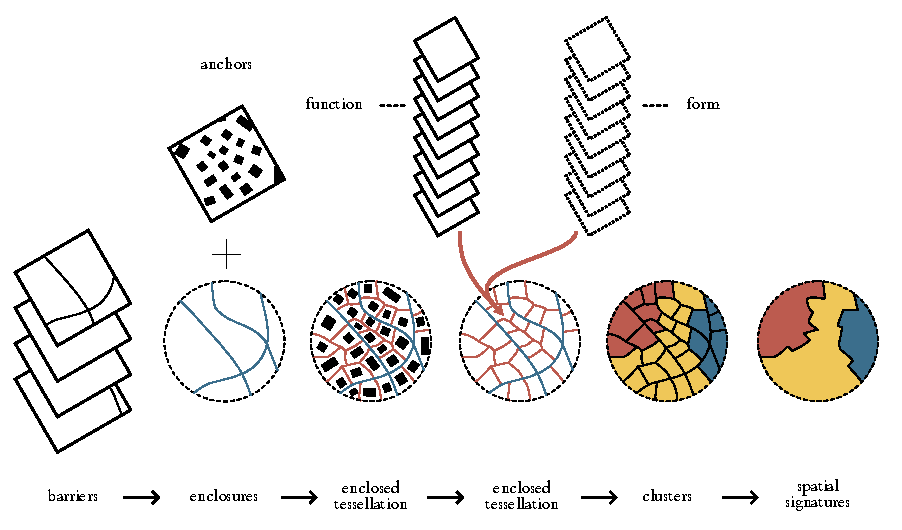
\includegraphics[width=\linewidth]{fig/workflow.pdf}
\caption{Diagram illustrating the sequential steps leading to the delineation of
spatial signatures. From a series of enclosing components, to enclosures,
enclosed tessellation (ET), the addition of form and function characters to ET
cells, and the development of spatial signatures.}
\label{fig:workflow}
\end{figure}

    % In this paper
% Great British Signatures
We introduce an open data product (ODP \cite{odp_paper21}) containing a classification of
spatial signatures for Great Britain (illustrated in a figure \ref{fig:map}). In doing so, we provide an
analysis-ready layer that brings together urban form and function consistently, in
detail, and at national scale. To the best of our knowledge, this is the first
dataset capturing urban form and function published both with a degree of detail and scale as
ours.
%% Input data used
Our results are based on the analysis of more than 14 million of ETCs, to
each of which we attach more than 300 characters capturing a wide range of
aspects relating to urban form and function.
%% Data available
We provide access to both granular geographical boundaries of the delineated spatial signatures
as well as measurements for each character at the signature level.
%% Web map and code
The ODP also includes a web map that allows exploration without any technical
requirement other than a web browser, and we have open sourced all the code,
including details on the computational backend.
%% Comparison with other datasets
The uniqueness of our ODP makes it challenging to set up a technical validation as a
comparison with existing datasets. Nevertheless, we relate our
signatures to a few well-established data products that capture each a subset
of the form and function dimensions we consider. Our results are encouraging
in that they show broad agreement in expected areas, but also highlight
aspects that can only be discovered when considering form and function in tandem.


\begin{figure}
    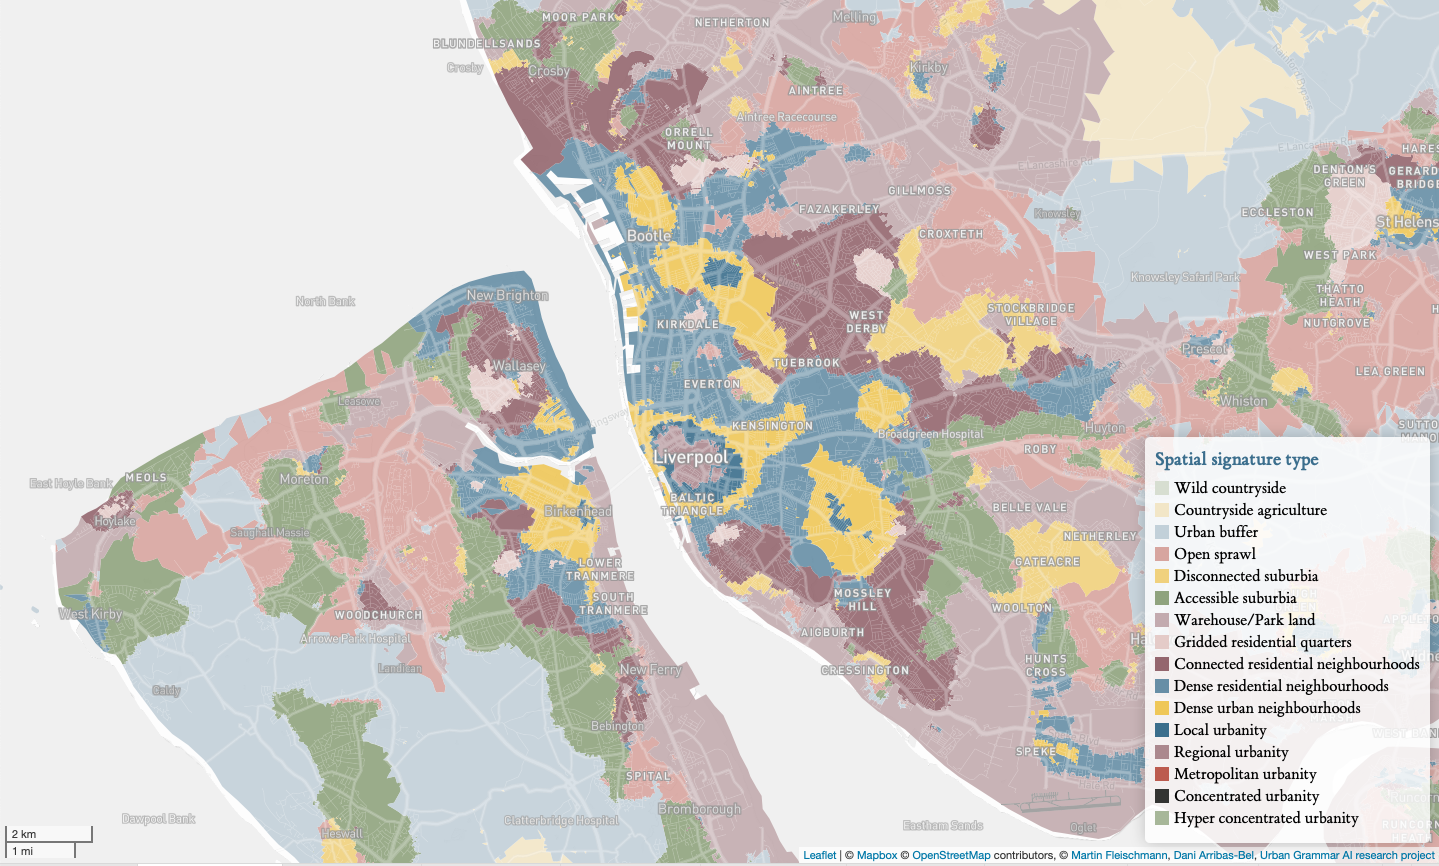
\includegraphics[width=\linewidth]{fig/signatures_map.png}
\caption{Illustration of a classification of spatial signatures in Liverpool and
    Birkenhead area, in the north west of England.}
\label{fig:map}
\end{figure}

% Benefits of signature approach (goals why we created it)
The approach and outputs presented bring several benefits to a range of
stakeholders interested in cities.
%% ODP
This spatial signatures ODP provides insight generated from detailed,
comprehensive and computationally intensive data analysis and presents it in a
way that is easy to access, work with and integrate into larger projects.
%
%%% Academics and policymakers
Together with the importance of form and function discussed above, we
anticipate the output will be relevant to both academic researchers as well as
policymakers and practitioners.
%% Broader SS benefits
As a conceptual framework, the spatial signatures provide a flexible yet
generalisable approach to understand, characterise and quantify urban form and
function. One way to understand our results is as an implementation of a
more general way of thinking about the spatial dimension of cities. In this
context, it can be useful to researchers and practitioners who, even if not
specifically interested in Great Britain, would like to implement a similar
approach.

% emphasize how this data can be used for various analysis
To give an example, spatial signatures may be used to delineate types of

origin and destination locations in mobility analysis, that could unveil patterns

of commuting or migration in extreme situations like the COVID-19 pandemics and
hypothetised \textit{flee from the city}. Another application may focus on equality
of access to services and amenities within the UKs Levelling Up agenda and target
areas based on their signature type, knowing that they will share key structural
components. At the same time, we do not expect signatures to focus on a single
aspect of urban environment as e.g. Local Climate Zones \citep{stewart2012local}
focusing primarily on assessment of climate would, but expect a wider range of
uses due to their inclusion of both form and function and a data driven nature reflecting
the specific place rather than abstract conceptual classes.

%
In this respect, we hope the present paper serves not only to document our own
work but to inspire future efforts aimed at urban form and function.



            %%% FROM ORIGNAL GUIDELINE %%%

% An overview of the study design, the assay(s) performed, and the created data, including any background information needed to put this study in the context of previous work and the literature.

%- Briefly outline the broader goals that motivated the creation of this dataset and the potential reuse value.

%- We also encourage authors to include a figure that provides a schematic overview of the study and assay(s) design.


